%!TEX program = xelatex
%!TEX TS-program = xelatex
%!TEX encoding = UTF-8 Unicode
%-*-coding : UTF-8 -*-
%main.tex
%
\documentclass[12pt]{article}  %设置文章总排版格式
\usepackage{url,fontspec,xltxtra,xunicode,graphicx,xeCJK,listings,float}
\setCJKmainfont{Songti SC}     % 设置中文字体
\setCJKmonofont{Songti SC}
\setromanfont{Times New Roman} % 设置英文字体
\newfontfamily\courier{Courier New}
\lstset{linewidth=1.1\textwidth,
        numbers=left, %设置行号位置 
        basicstyle=\small\courier,
        numberstyle=\tiny\courier, %设置行号大小  
        keywordstyle=\color{blue}\courier, %设置关键字颜色  
        %identifierstyle=\bf,
        commentstyle=\it\color[cmyk]{1,0,1,0}\courier, %设置注释颜色 
        stringstyle=\it\color[RGB]{128,0,0}\courier,
        %framexleftmargin=10mm,
        frame=single, %设置边框格式  
        %backgroundcolor=\color[RGB]{0.1,0.1,0.76},
        %escapeinside=``, %逃逸字符(1左面的键),用于显示中文  
        breaklines, %自动折行  
        extendedchars=false, %解决代码跨页时,章节标题,页眉等汉字不显示的问题  
        xleftmargin=2em,xrightmargin=2em, aboveskip=1em, %设置边距  
        tabsize=4, %设置tab空格数  
        showspaces=false %不显示空格  
        basicstyle=\small\courier
       } 
\title{Tor项目扩展应用}
\author{Mod233}
\date{\today}
\XeTeXlinebreaklocale "zh"					   % 
\XeTeXlinebreakskip = 0pt plus 1pt minus 0.1pt %自动换行
\bibliographystyle{plain} %参考文献的格式

\begin{document}   %正文开始

\maketitle
\begin{abstract}
对于Tor的研究在大四上持续了半学期,可以说收获颇丰。Tor作为匿名网络的鼻祖,是我为我未来工作生活,提供匿名安全的有效工具。这里我会就Tor配置、Tor爬虫、Tor木马等方面展开。
\end{abstract}
\tableofcontents
\section{Tor配置} % (fold)
\label{sec:熟悉latex}
\ \ \ \ \ Tor环境配置,可以使用简单的Tor浏览器,或者CLI命令行界面。我这里主要以CLI展开,因为主要是为了后面章节导入爬虫、木马等等流量做铺垫。\par
如果不使用Tor浏览器,整个流程的配置,相对复杂。因为大陆会屏蔽Tor的流量,在Tor Browser中集成了meek-amazon 和meek-azure来绕过检测。但随着技术的慢慢进步,meek作为跳板肯定不是长久之计,所以这里介绍结合 Shadowsocks、Tor、Privoxy来实现匿名服务的系统。 \par
基本网络拓扑如下: \par

\begin{figure}[h]
\centering
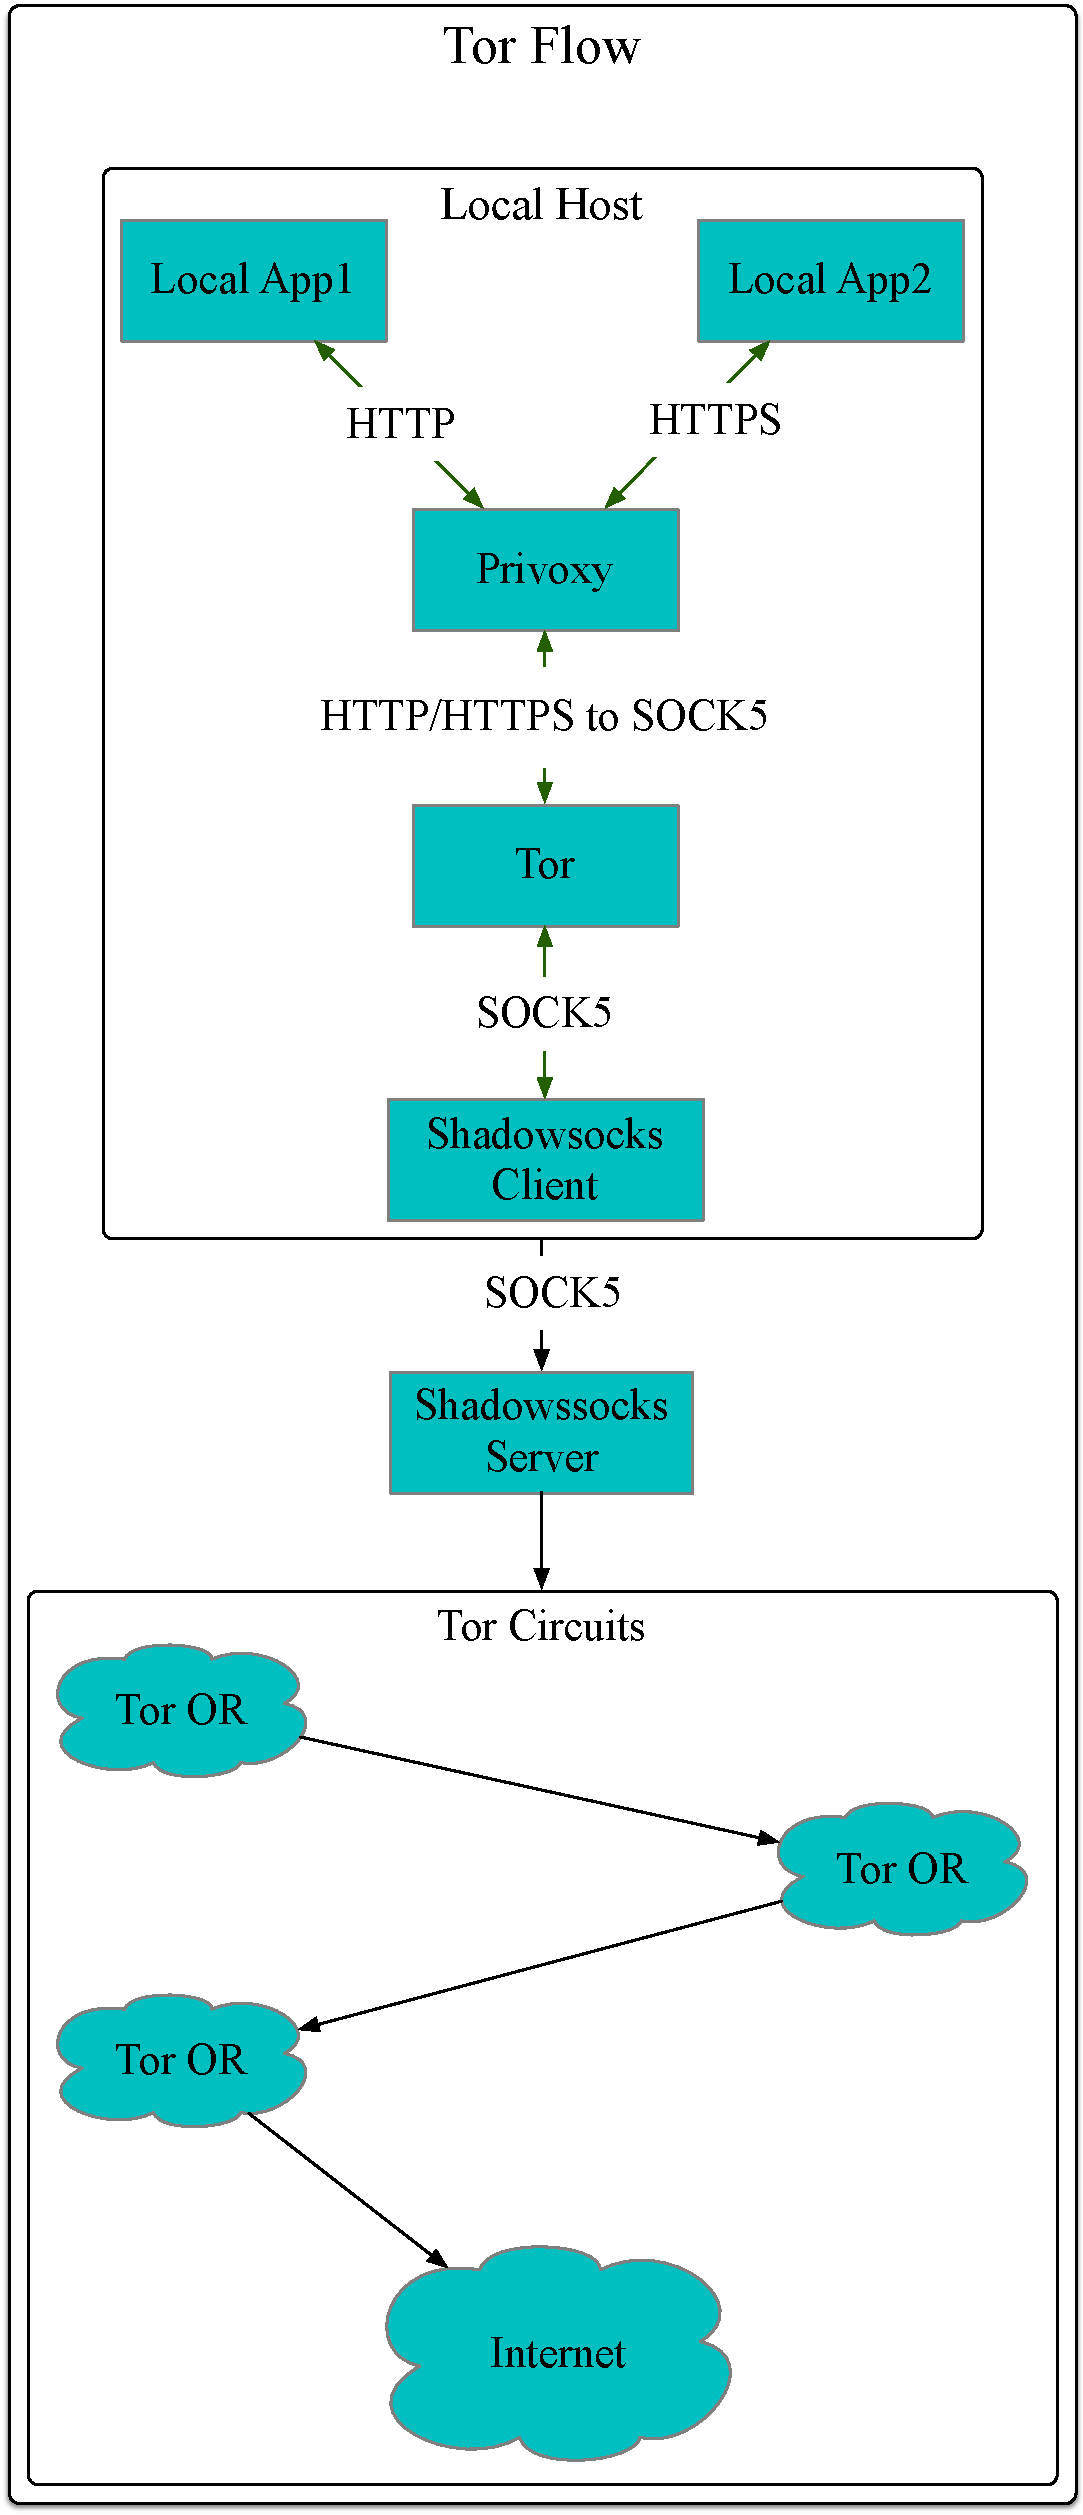
\includegraphics[scale=0.3]{pic/tor2.pdf}
\end{figure}

\par
从拓扑中,可以看出,主要是Privoxy实现HTTP/HTTPS到SOCK5的转换,然后又Tor封装一层后,交给Shadowsocks Client,然后由Shadowsocks Client将数据包传给处于境外端口的Shadowsocks Server,这个Server节点能访问Tor的节点IP并且不会被拦截,流量就成功接入了Tor网络中。
下面逐个介绍 Privoxy,Tor,Shadowsocks的环境配置情况。
\par
首先是Privoxy:
\begin{lstlisting}[language=sh]
➜  ~ brew install privoxy
➜  ~ cd /usr/local/etc/privoxy
➜  privoxy ls
config           default.filter   templates        user.action
default.action   match-all.action trust            user.filter
➜  privoxy cat config
...SNIP...
listen-address  127.0.0.1:8118
forward-socks5 / 127.0.0.1:9050
forward-socks5t / 127.0.0.1:9050     #socks5-tor
forward-socks   / 127.0.0.1:9050
...SNIP...
➜  privoxy sudo /Applications/Privoxy/startPrivoxy.sh
➜  privoxy sudo /Applications/Privoxy/stopPrivoxy.sh
\end{lstlisting}
\par
Privoxy中,listen-address,指名了监听的ip及port,forward指明了转发规则。完成了privoxy的配置后,可以登陆\emph{http://config.privoxy.org/}进行测试:
\begin{figure}[h]
\centering
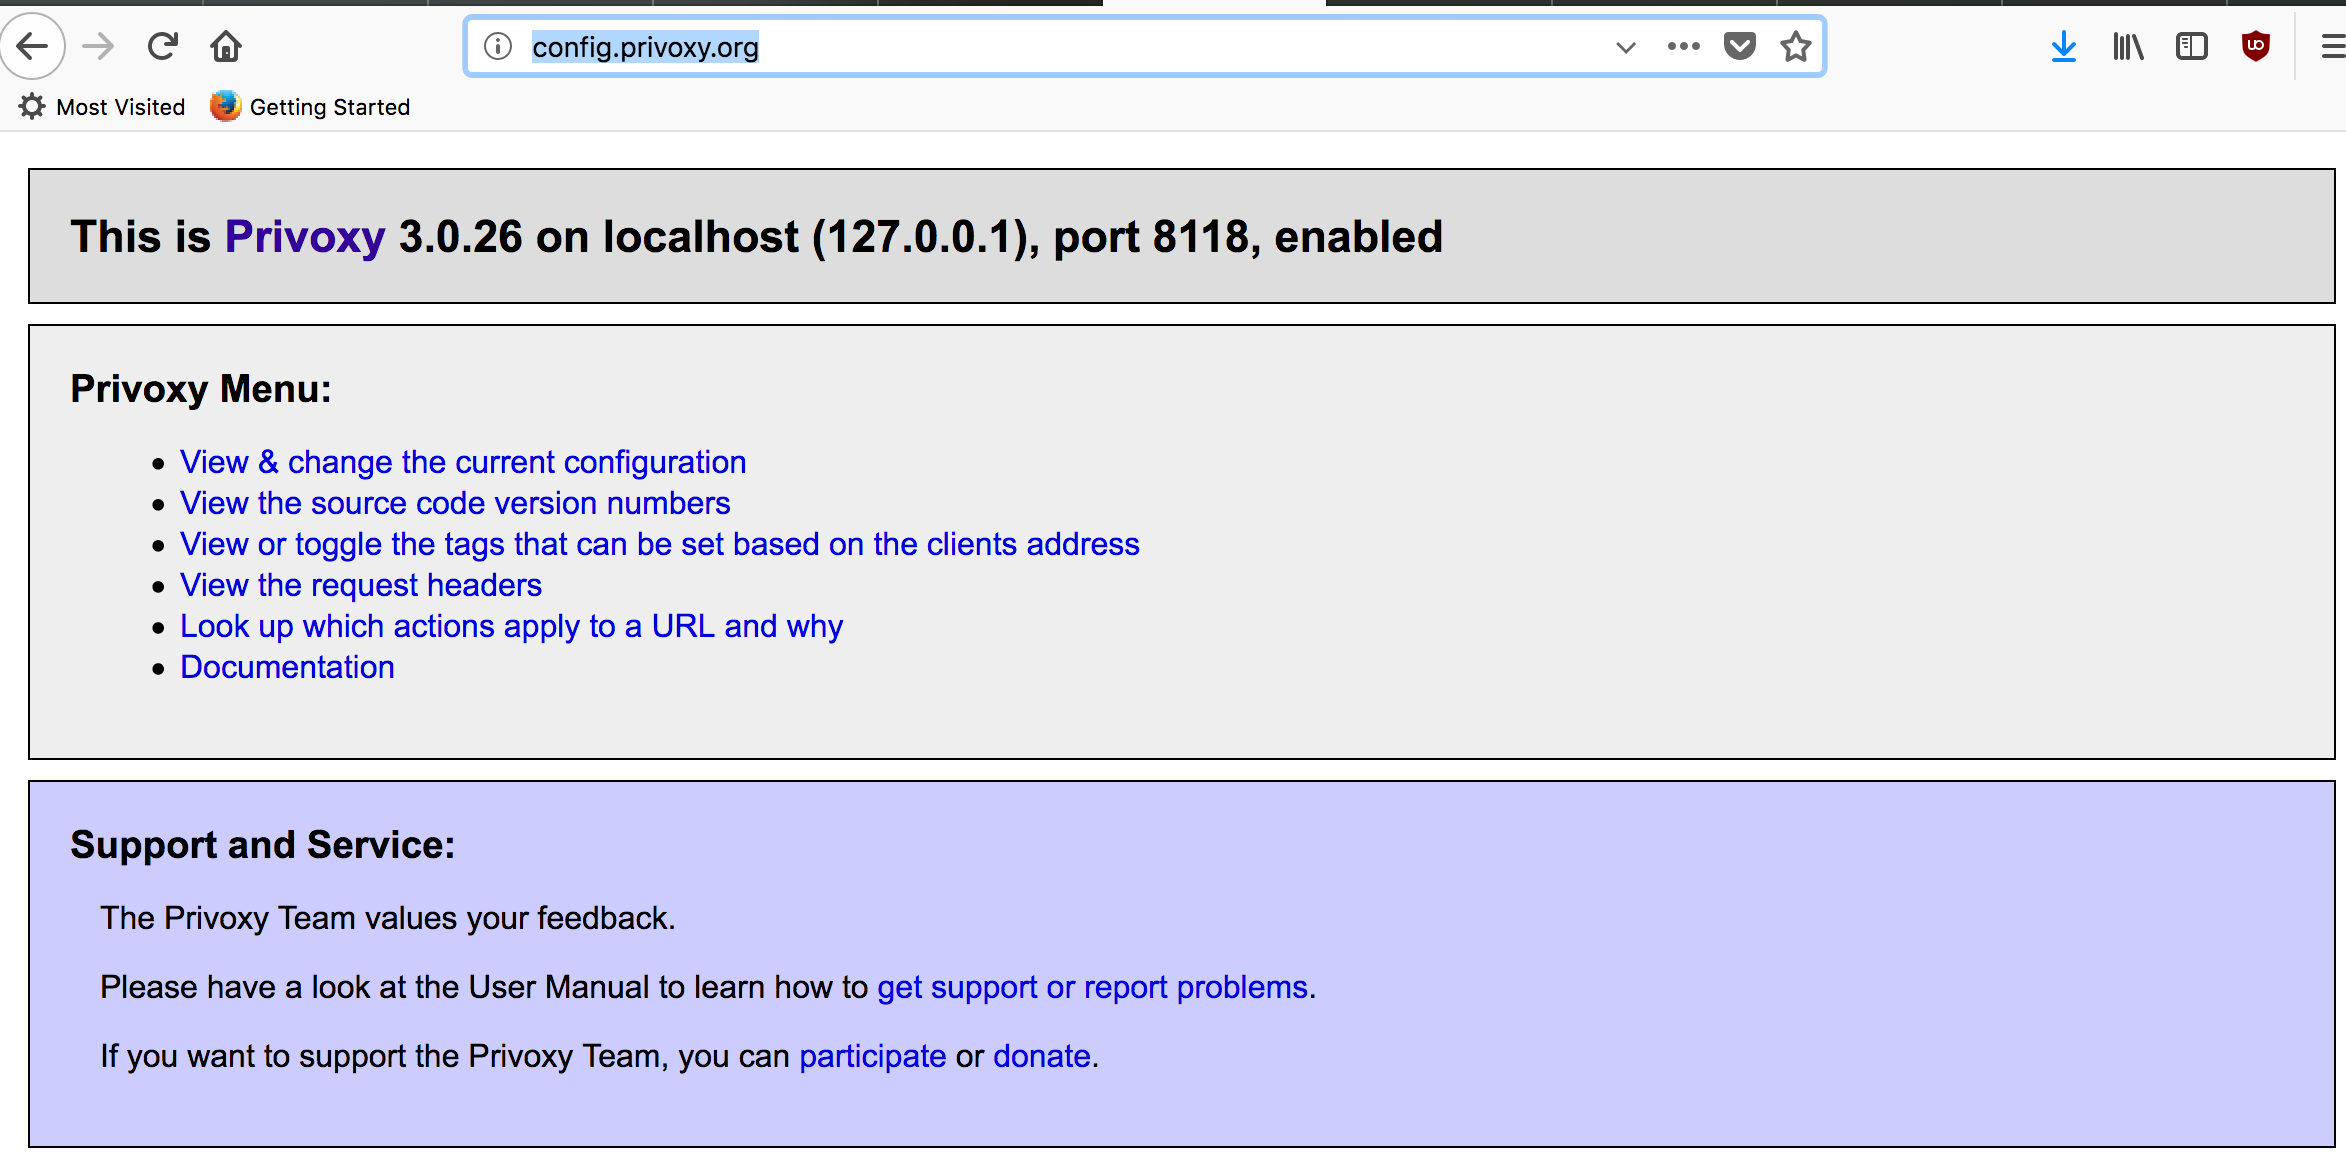
\includegraphics[scale=0.3]{pic/privoxy.png}
\end{figure}
\par
接下来需要下载Tor源码,并编译安装,源代码从官网(https://www.torproject.org/download/download.html.en)下载即可,一般类Unix系统都会有对用的包管理器提供快速的安装:

\begin{lstlisting}[language=sh]
➜  CodeTor-0.3.3.7 brew install tor
...SNIP...
To have launchd start tor now and restart at login:
  brew services start tor
Or, if you don't want/need a background service you can just run:
  tor
==> Summary
🍺  /usr/local/Cellar/tor/0.3.3.7: 21 files, 11.2MB
...SNIP...
➜  ~ cd /usr/local/etc/tor
➜  tor ls
torrc
➜  tor cat torrc
...SNIP...
Socks5Proxy 127.0.0.1:1077
SocksPort 9050
ControlPort 9051
➜  tor -f /usr/local/etc/tor/torrc
\end{lstlisting}
\par
之后需要到\ \emph{/usr/local/tor/}\ 文件夹下,修改配置文件,改成如上的情况即可。之后利用启动即可。


\par
配置shadowsocks环境,网上已经有非常多教程了,而且shadowsocks在整个系统中相当于流量转发的功能,这里不赘述了。想要测试shadowssocks是否成功,可以尝试下面的命令,如果返回ss-server的地址,则说明配置成功:
\begin{lstlisting}[language=sh]
➜  ~ curl --socks5 127.0.0.1:1077 http://httpbin.org/ip
{"origin":"95.163.200.165"}
\end{lstlisting}
\par
接下来是浏览器的配置,如果自己是firefox浏览器,在浏览器\  \emph{preference->setting}\  配置对应的代理服务即可:
\begin{figure}[H]
\centering
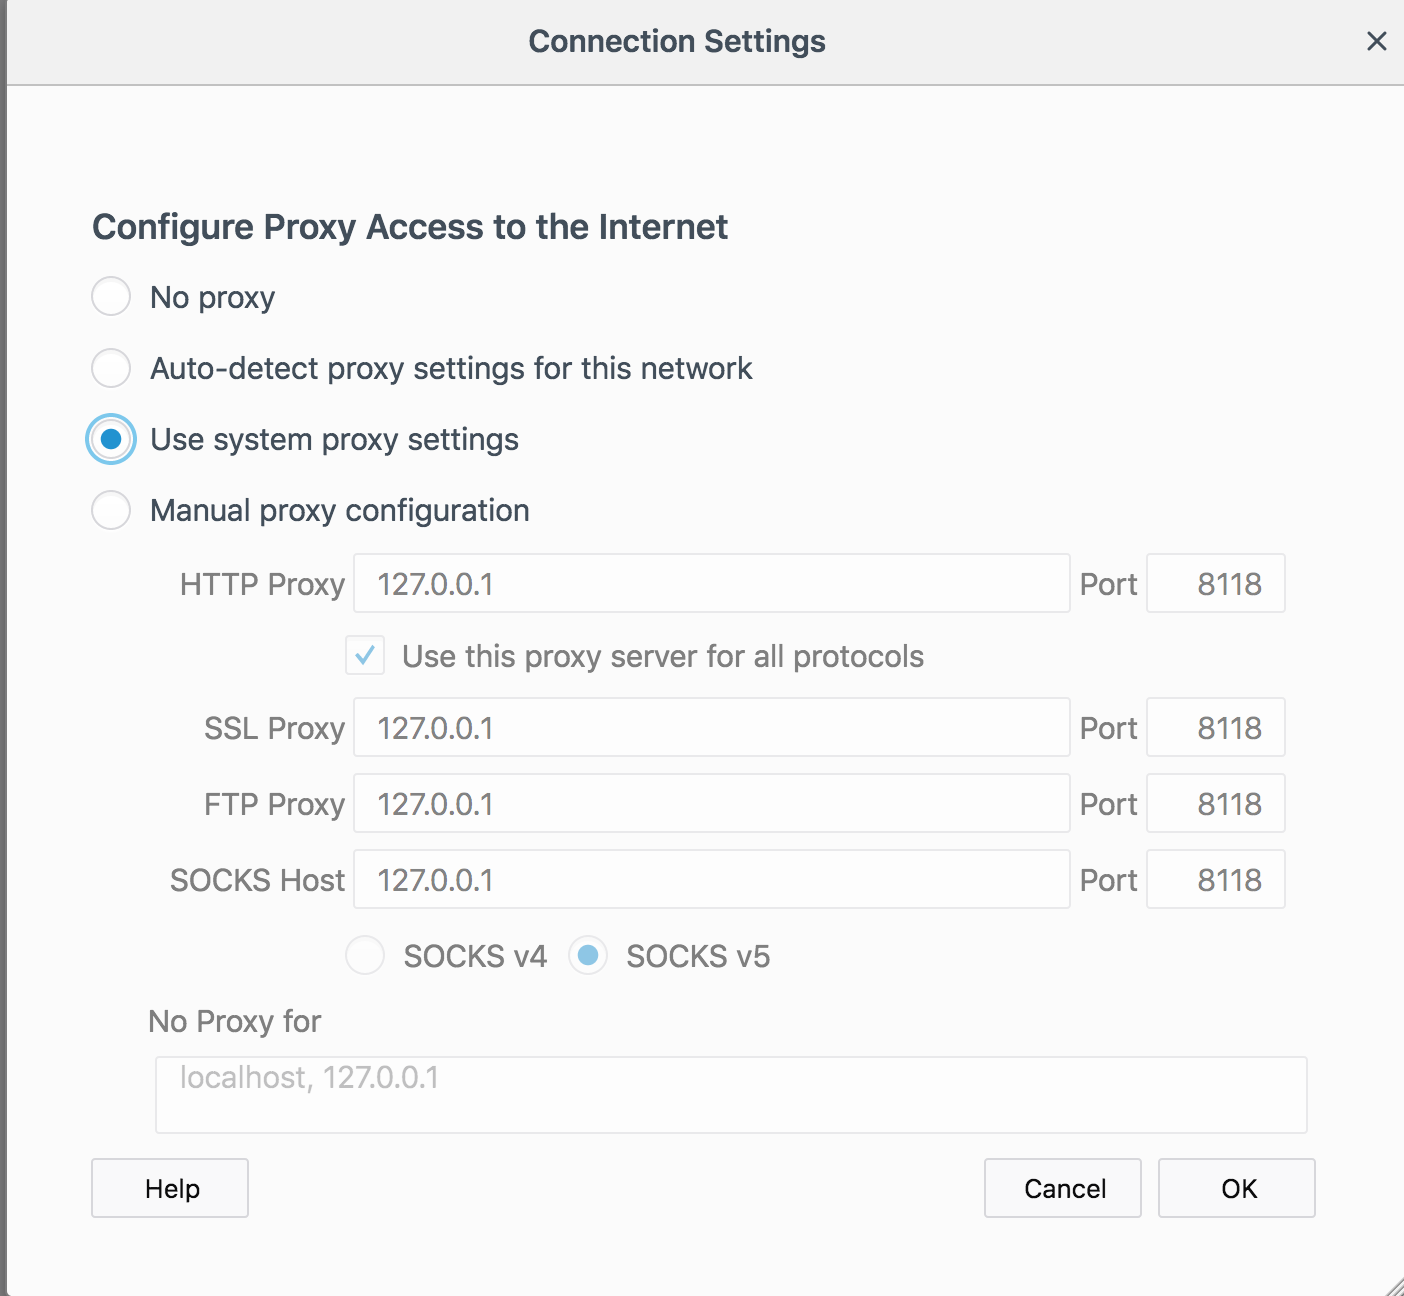
\includegraphics[scale=0.3]{pic/proxy.png}
\end{figure}
\par
Tor提供了一个测试网站,供用户测试流量是否经过了Tor网络,登陆\ \emph{https://check.torproject.org/} \ 访问即可:
\begin{figure}[H]
\centering
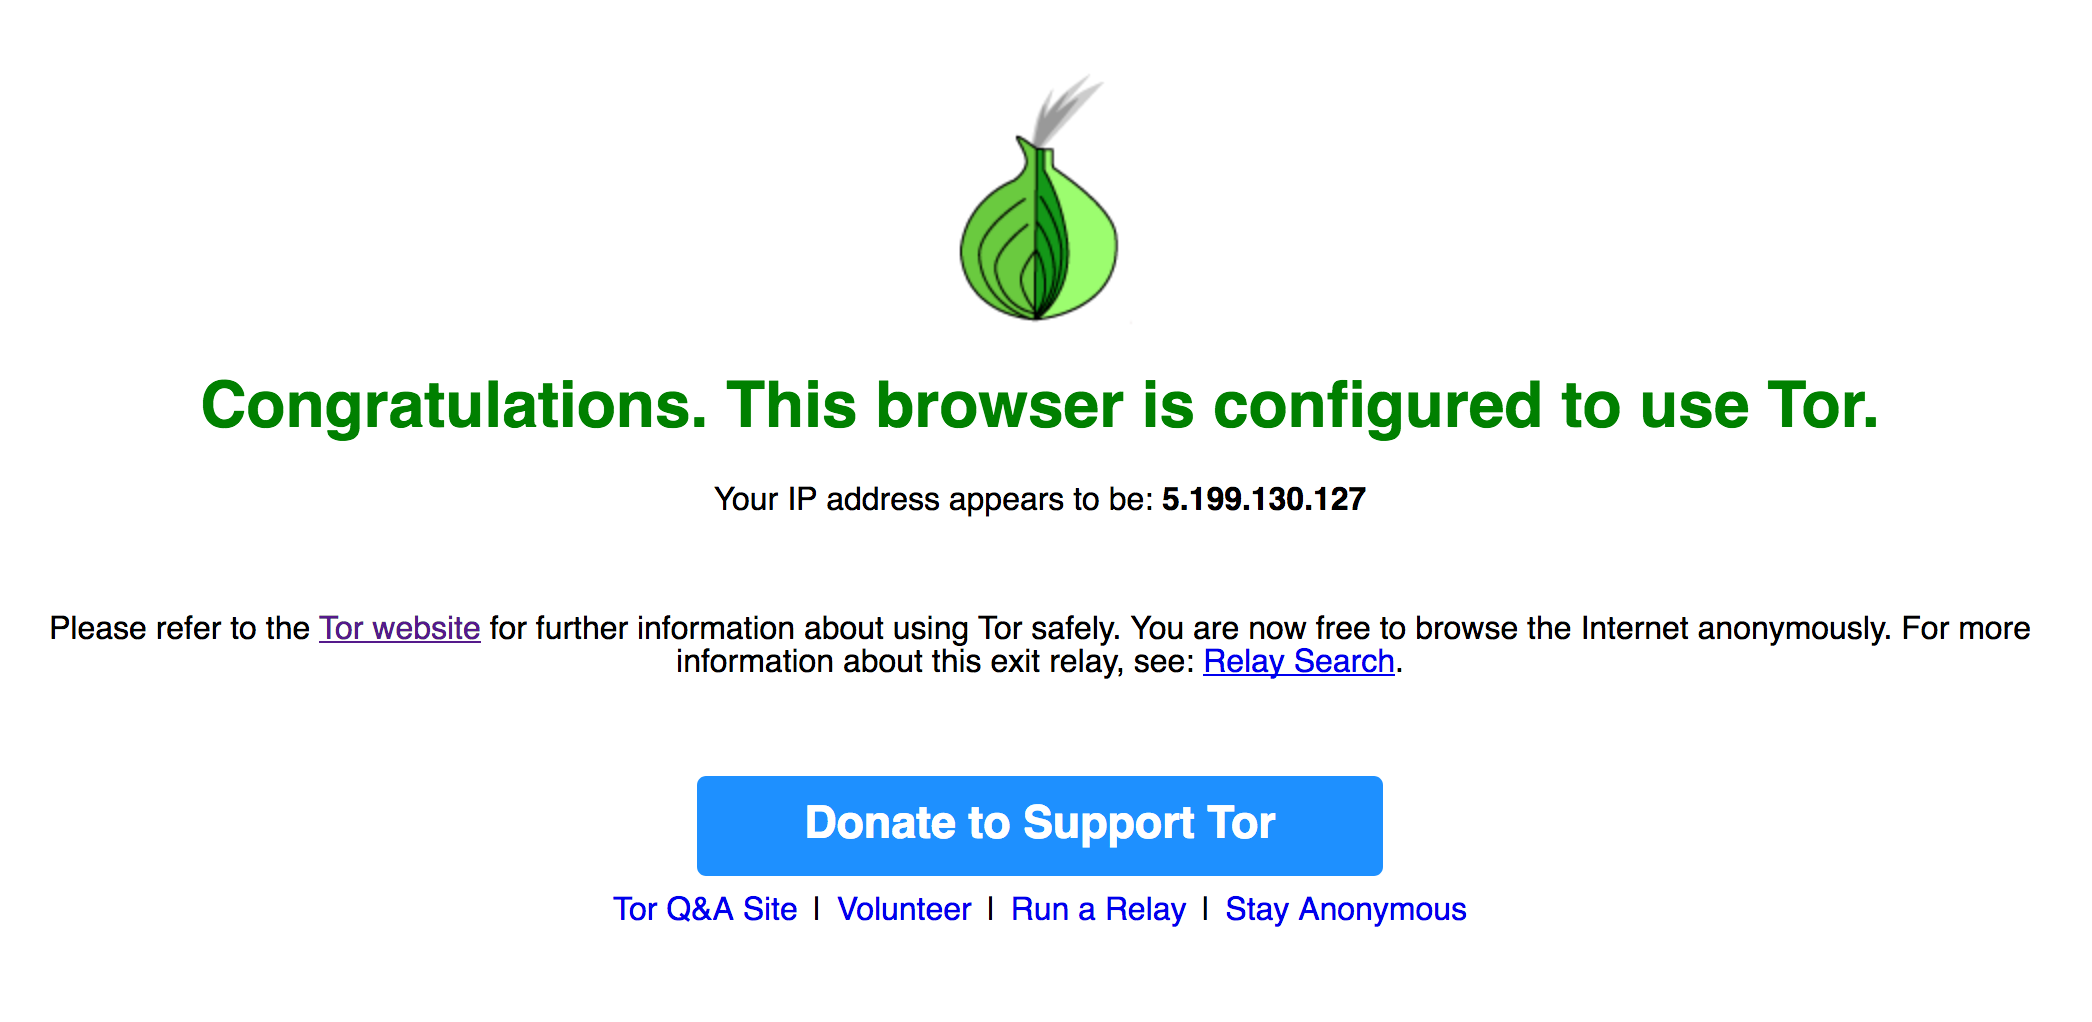
\includegraphics[scale=0.3]{pic/succed.png}
\end{figure}
\section{Tor认证原理} % (fold)
\label{sec:组织你的文本}
\ \ \ \ \ 仔细想想,Tor有很多值得自己推敲的问题。比如为什么Tor选择Socks协议,为什么Tor能够防追踪。
\section{Tor爬虫} % (fold)
\label{sec:自动化工具}
\ \ \ \ \ Tor爬虫有两种理解,一种是指利用Tor特性中IP动态调变的优势,以不同的IP动态爬取网页信息,而不会因为单个IP频发访问遭到屏蔽;
另一种是通过Tor进入暗网,爬取暗网中的数据。
\section{玩转数学公式} % (fold)
\label{sec:玩转数学公式}
b
\section{绘制图表} % (fold)
\label{sec:绘制图表}
\section{幻灯片演示} % (fold)
\label{sec:幻灯片演示}
\section{从错误中救赎} % (fold)
\label{sec:从错误中救赎}
\section{Latex无极限} % (fold)
\label{sec:Latex无极限}

% section section_name (end)
\end{document} %正文结束